\documentclass{beamer}
\usepackage[orientation=landscape,size=a0,scale=1.2]{beamerposter}
\usepackage{haziq_poster}
\usepackage{haziq_maths}

%%%%%%%%%%%%%%%%%%%%%%%%%%%%%%%%%%%%%%%%%%%%%%%%%%%%%%%%%%%%%%%%%%%%%%%%%%%%%%%%
%%% POSTER SETTINGS %%%%%%%%%%%%%%%%%%%%%%%%%%%%%%%%%%%%%%%%%%%%%%%%%%%%%%%%%%%%
%%%%%%%%%%%%%%%%%%%%%%%%%%%%%%%%%%%%%%%%%%%%%%%%%%%%%%%%%%%%%%%%%%%%%%%%%%%%%%%%
\setbeamercolor{block title}{fg=black,bg=white}
\setbeamercolor{block body}{fg=black,bg=white}
\setbeamercolor{block alerted title}{fg=white,bg=black}
\setbeamercolor{block alerted body}{fg=black,bg=white}

% Define the column widths and overall poster size
% To set effective sepwid, onecolwid and twocolwid values, first choose how many columns you want and how much separation you want between columns
% In this template, the separation width chosen is 0.024 of the paper width and a 4-column layout
% onecolwid should therefore be (1 - sepwid * (# of columns + 1)) / # of columns 
% e.g. (1 - 0.024 * (4 + 1)) / 4 = 0.22
% Set twocolwid to be (2 * onecolwid) + sepwid = 0.464
% Set threecolwid to be (3 * onecolwid) + 2 * sepwid = 0.708
% The whole poster consists of three major columns, the second of which is split into two columns twice - the [t] option aligns each column's content to the top
% A0 is 841 x 1189 mm
% sep      =  28.536 mm
% half sep =  14.268 mm
% onecol   = 261.580 mm
% total    = 304.384 mm
\newlength{\sepwid}
\newlength{\onecolwid}
\newlength{\twocolwid}
\newlength{\threecolwid}
\setlength{\sepwid}{0.024\paperwidth} % Separation width (white space) between columns
\setlength{\onecolwid}{0.22\paperwidth} % Width of one column
\setlength{\twocolwid}{0.464\paperwidth} % Width of two columns
\setlength{\threecolwid}{0.708\paperwidth} % Width of three columns

% Title section
\title{
  Regression Modelling with Priors using Fisher Information\\[0.4ex] 
  Covariance Kernels (I-priors)
}

\author{Haziq Jamil}

\institute{
  Department of Statistics\\
  London School of Economics and\\[0.3ex] 
  Political Science\\[0.7ex]
  \url{http://haziqj.ml}
}

%%%%%%%%%%%%%%%%%%%%%%%%%%%%%%%%%%%%%%%%%%%%%%%%%%%%%%%%%%%%%%%%%%%%%%%%%%%%%%%%
%%% BEGIN DOCUMENT %%%%%%%%%%%%%%%%%%%%%%%%%%%%%%%%%%%%%%%%%%%%%%%%%%%%%%%%%%%%%
%%%%%%%%%%%%%%%%%%%%%%%%%%%%%%%%%%%%%%%%%%%%%%%%%%%%%%%%%%%%%%%%%%%%%%%%%%%%%%%%
\begin{document}
\begin{frame}[t]  % the whole poster is enclosed in one beamer frame
\vspace{-0.3cm}
\begin{columns}[t]  % and in the columns environment

% Draw lines separating columns
\tikz[remember picture,overlay]{\draw[black,thick] ([shift={(4mm,-35.8cm)}]current page.north) -- ([shift={(4mm,1.6cm)}]current page.south);}
\tikz[remember picture,overlay]{\draw[black,thick] ([shift={(308mm,-11.5cm)}]current page.north west) -- ([shift={(308mm,1.6cm)}]current page.south west);}
\tikz[remember picture,overlay]{\draw[black,thick] ([shift={(-301mm,-11.5cm)}]current page.north east) -- ([shift={(-301mm,1.6cm)}]current page.south east);}

%%%%%%%%%%%%%%%%%%%%%%%%%%%%%%%%%%%%%%%%%%%%%%%%%%%%%%%%%%%%%%%%%%%%%%%%%%%%%%%%
%%% FIRST COLUMN %%%%%%%%%%%%%%%%%%%%%%%%%%%%%%%%%%%%%%%%%%%%%%%%%%%%%%%%%%%%%%%
%%%%%%%%%%%%%%%%%%%%%%%%%%%%%%%%%%%%%%%%%%%%%%%%%%%%%%%%%%%%%%%%%%%%%%%%%%%%%%%%
\spacercolumn
\begin{column}{\onecolwid} % The first column

\vspace{-0.6cm}
\begin{figure}[t]
  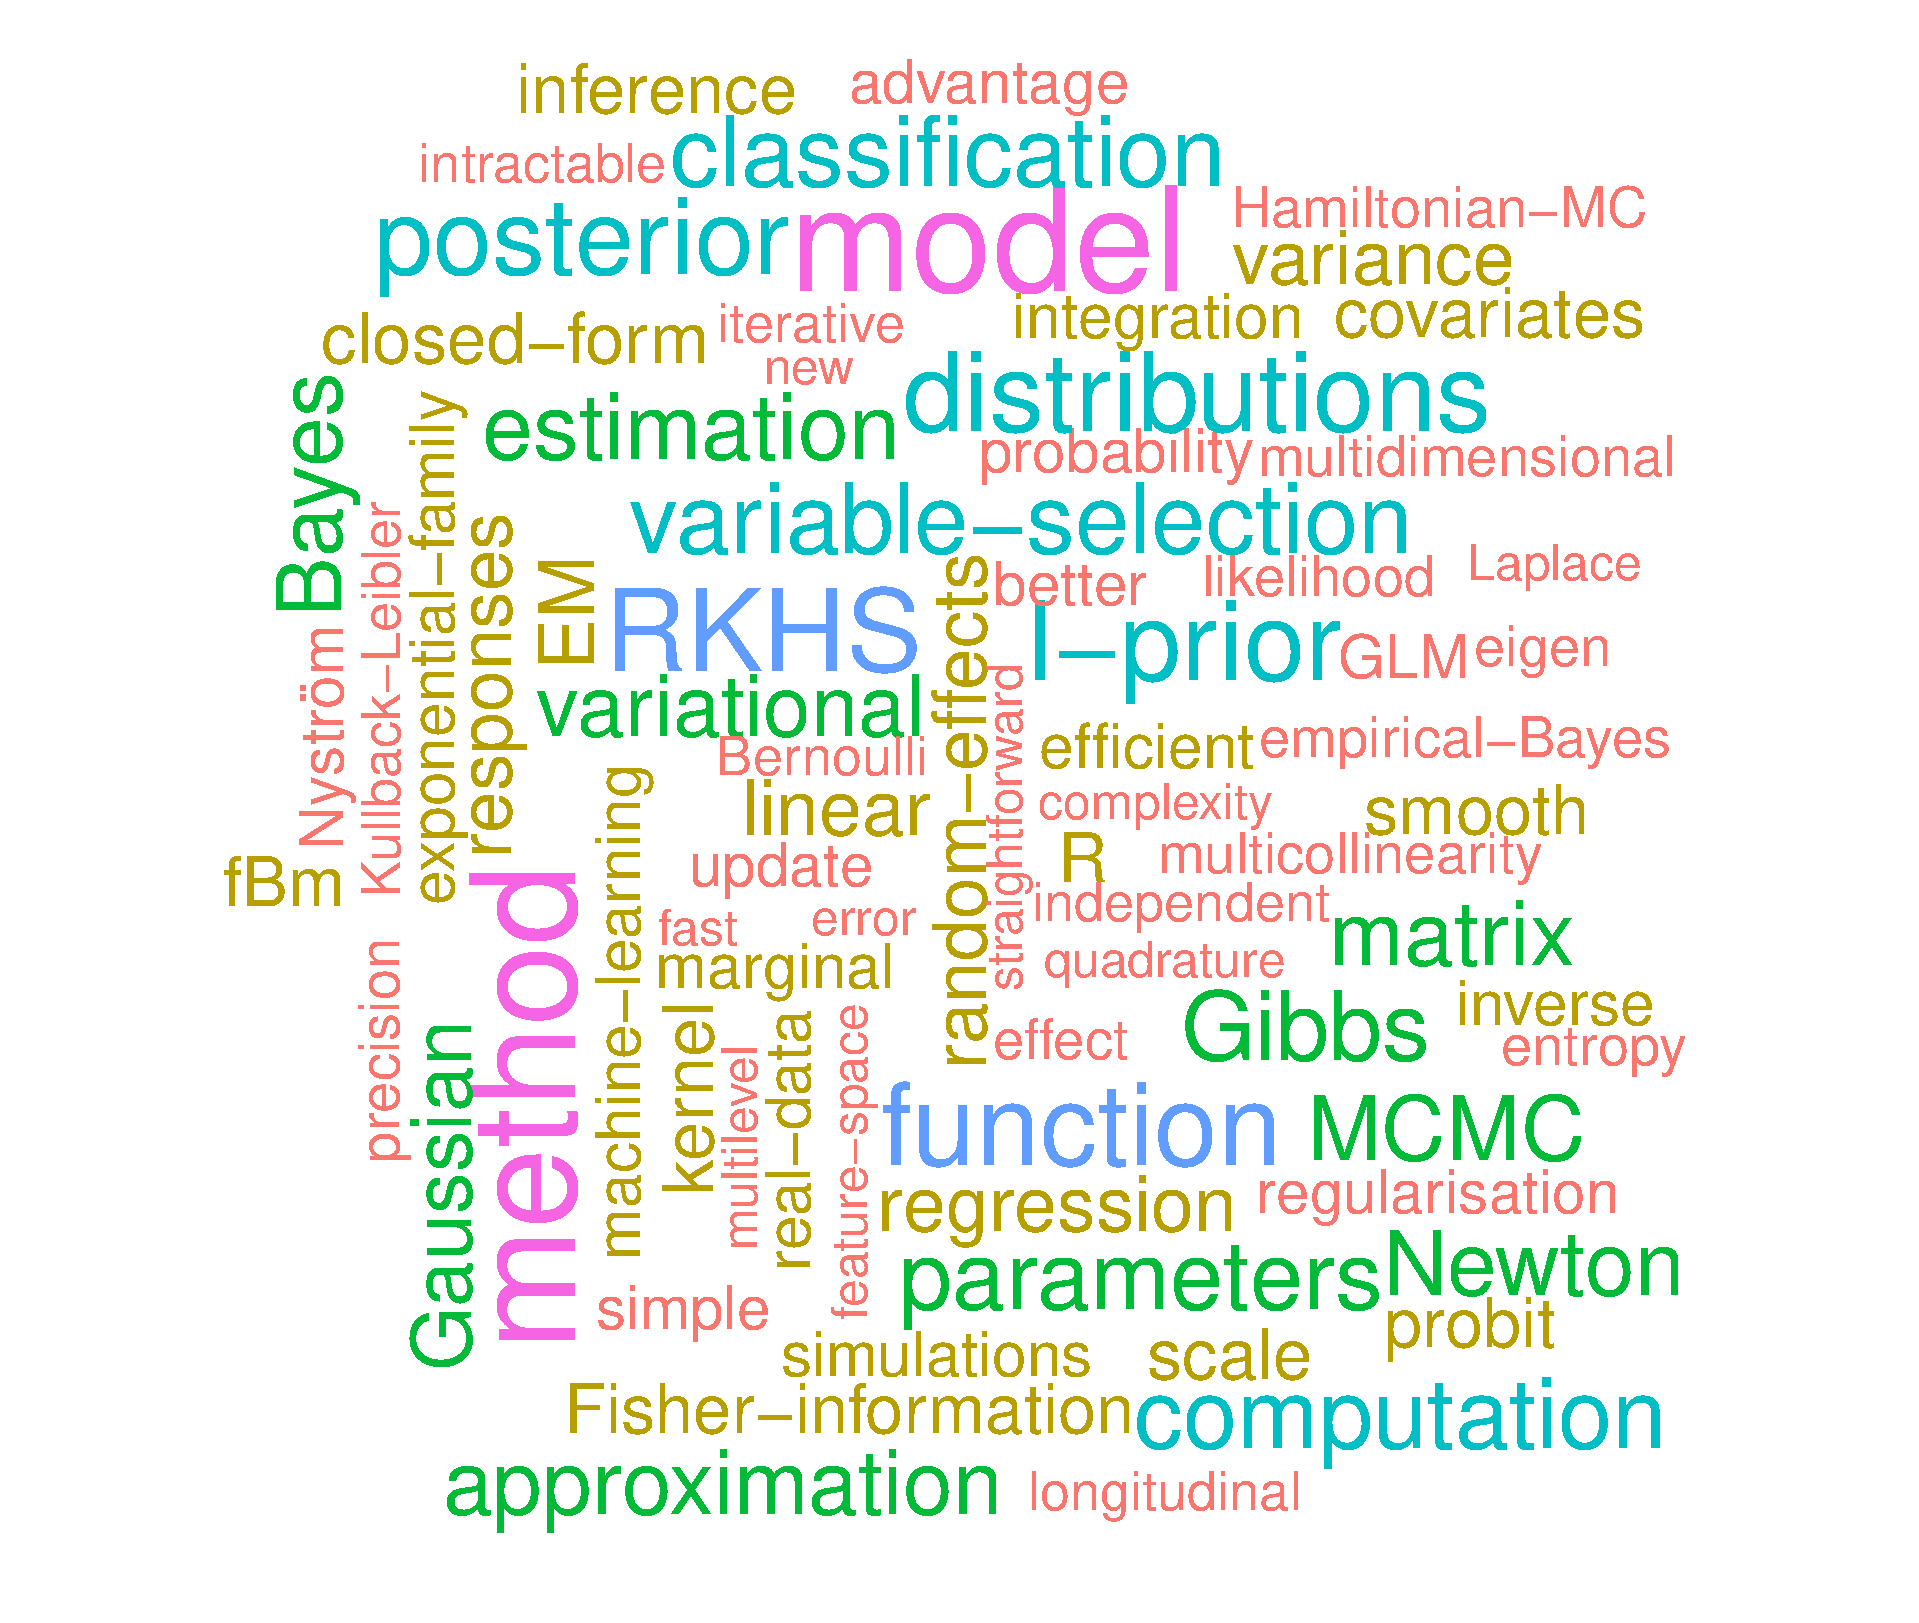
\includegraphics[width=\linewidth]{figure/keyword.png}
\end{figure}

%% Objectives ------------------------------------------------------------------
%\setbeamercolor{block alerted title}{fg=white,bg=colgrey} % Change the alert block title colors
%\setbeamercolor{block alerted body}{fg=black,bg=white} % Change the alert block body colors
%
%\begin{alertblock}{Objectives}
%
%\begin{itemize}
%  \item Outline an efficient computational method for estimating the parameters of an I-prior model in the continuous responses case.
%  \item Extend the I-prior methodology to categorical responses for classification and inference.
%  \item Explore the usefulness of I-priors towards variable selection.
%\end{itemize}
%
%\end{alertblock}


% Introduction -----------------------------------------------------------------
\begin{block}{Introduction}

Consider the following regression model for $i=1,\dots,n$:
~\\[-20pt]
\begin{align}\label{eq:normalmodel}
  \begin{gathered}
      y_i = f(x_i) + \epsilon_i \\
    (\epsilon_1, \dots, \epsilon_n)^\top \sim \N_n(0,\Psi^{-1})
  \end{gathered}
\end{align}
~\\[-7pt]
where $y_i \in \bbR$, $x \in \cX$, and $f \in \cF$. Let $\cF$ be a reproducing kernel Hilbert space (RKHS) with kernel $h_\lambda:\cX \times \cX \to \bbR$. The Fisher information for $f$ evaluated at $x$ and $x'$ is
~\\[-20pt]
\begin{align}
  \cI\big(f(x), f(x')\big) = \sum_{k=1}^n \sum_{l=1}^n \Psi_{k,l} h_\lambda(x,x_k) h_\lambda(x',x_l).
\end{align}

\setbeamercolor{block alerted title}{fg=white,bg=colgrey} % Change the alert block title colors
\setbeamercolor{block alerted body}{fg=black,bg=white} % Change the alert block body colors
\begin{alertblock}{The I-prior}

The entropy maximising prior distribution for $f$, subject to constraints, is 
%Gaussian with mean chosen \emph{a priori}, and covariance equal to the Fisher information for $f$.
\[
  \bff = \big(f(x_1),\dots,f(x_n) \big)^\top \sim \N_n \big(\bff_0, \cI[f] \big).
\]

\vspace{10pt}

\end{alertblock}

\vspace{-10pt}
Of interest are 

\newcommand{\new}{{\text{new}}}
\begin{itemize}
  \item the posterior distribution for the regression function
  \[
    p(\bff|\by) = \frac{p(\by|\bff) p(\bff)}{\int p(\by|\bff) p(\bff) \d \by}; \text{and}
  \]
  \item the posterior predictive distribution given new data
  \[
    p(y_\new|\by) = \int p(y_\new|f_\new,\by) p(f_\new|\by) \d f_\new.
  \]
\end{itemize}

\end{block}



% Estimation -------------------------------------------------------------------
\vspace{-20pt}
\begin{block}{Estimation}

Model parameters (error precision $\Psi$, RKHS scale parameters $\lambda$, and any others) may be estimated via

\begin{itemize}
  \item Maximum marginal likelihood, a.k.a. empirical Bayes;
  \item Expectation-maximisation (EM) algorithm; or
  \item Markov chain Monte Carlo (MCMC) methods.
\end{itemize} 

Under the normal model \eqref{eq:normalmodel}, the posterior for $y$, given some $x$ and model parameters, is normal with mean
~\\[-21pt]
\begin{gather}
  \hat y(x) = f_0(x) + \bh_\lambda^\top(x) \Psi H_\lambda
  \big(H_\lambda \Psi H_\lambda + \Psi^{-1}\big)^{-1}
  \big(y - f_0(x)\big) \nonumber \\
  \nonumber \\[-19pt]
  \beforetext{and variance} \label{eq:postmeanvar} \\
  \nonumber \\[-24pt]
  \hat\sigma^2(x) = \bh_\lambda^\top(x) 
  \big(H_\lambda \Psi H_\lambda + \Psi^{-1}\big)^{-1} 
  \bh_\lambda(x) + v_x \nonumber,
\end{gather}
~\\[-25pt]
where $v_x$ is some prior variance component.


\end{block}

\end{column}  % End of the first column



%%%%%%%%%%%%%%%%%%%%%%%%%%%%%%%%%%%%%%%%%%%%%%%%%%%%%%%%%%%%%%%%%%%%%%%%%%%%%%%%
%%% SECOND & THIRD COLUMNS %%%%%%%%%%%%%%%%%%%%%%%%%%%%%%%%%%%%%%%%%%%%%%%%%%%%%
%%%%%%%%%%%%%%%%%%%%%%%%%%%%%%%%%%%%%%%%%%%%%%%%%%%%%%%%%%%%%%%%%%%%%%%%%%%%%%%%
\spacercolumn
\begin{column}{\twocolwid}  % columns that is two columns wide



% I-prior figures --------------------------------------------------------------
\vspace{-1.8cm}
\begin{figure}
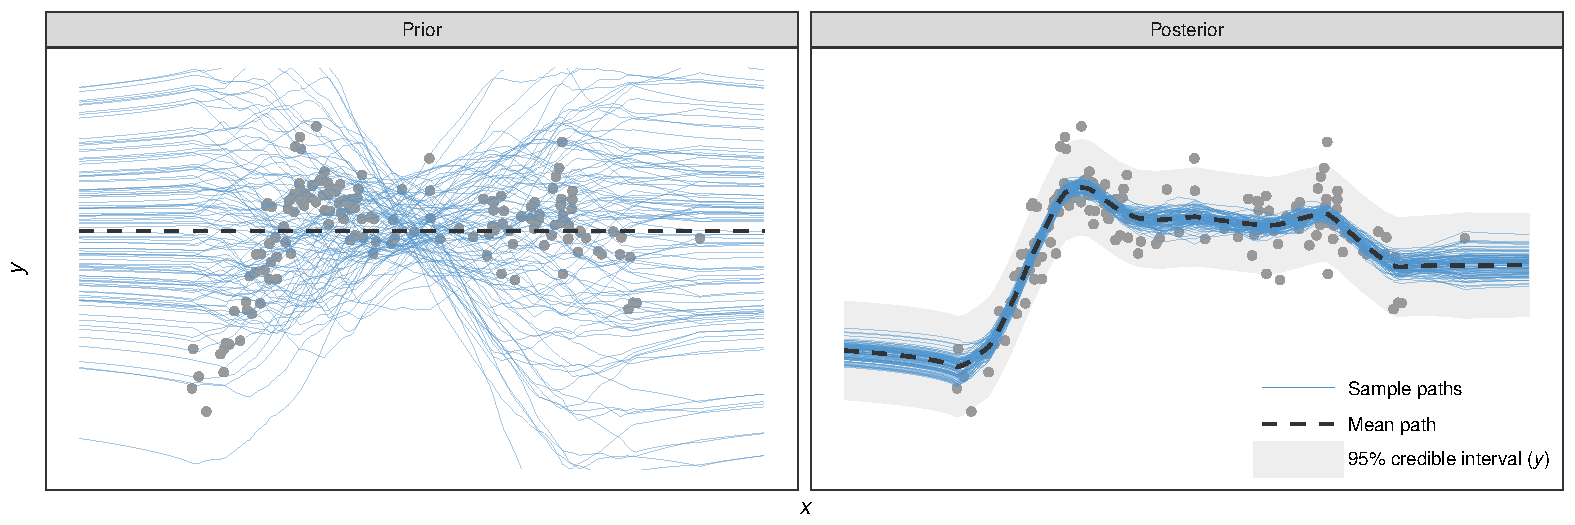
\includegraphics[width=\linewidth, height=20cm]{figure/iprior_function}
\vspace{-1.8cm}
\caption{Sample paths from the fractional Brownian motion RKHS under an I-prior (left) and the posterior (right). There is somewhat controlled behaviour at the boundaries (compared to Gaussian process priors, say). Fewer information in this region pulls the function estimate towards the prior mean. The 95\% credibility interval for posterior estimates of $y$ are shaded grey.}
\end{figure}



%%%%%%%%%%%%%%%%%%%%%%%%%%%%%%%%%%%%%%%%%%%%%%%%%%%%%%%%%%%%%%%%%%%%%%%%%%%%%%%%
%%% SECOND COLUMN %%%%%%%%%%%%%%%%%%%%%%%%%%%%%%%%%%%%%%%%%%%%%%%%%%%%%%%%%%%%%%
%%%%%%%%%%%%%%%%%%%%%%%%%%%%%%%%%%%%%%%%%%%%%%%%%%%%%%%%%%%%%%%%%%%%%%%%%%%%%%%%
\begin{columns}[t,totalwidth=\twocolwid]  % split the column
\begin{column}{\onecolwid}  % The first column within column 2 (column 2.1)



% Computational hurdles --------------------------------------------------------
\begin{block}{Computational Hurdle}

%For models with many scale parameters, 
%\begin{itemize}
%  \item Newton methods are problematic due to the presence of multiple local optima; while  
%  \item Gibbs sampling suffer from severe autocorrelation in the posterior samples.
%\end{itemize}
%The EM provides a reliable and straightforward framework for estimating the parameters of I-prior models.
%\\~\\[-0.8ex]
%Regardless, 
Computational complexity is dominated by the $n \times n$ matrix inversion in \eqref{eq:postmeanvar}, which is $O(n^3)$. Suppose that $H_\lambda = QQ^\top$, with $Q$ an $n \times q$ matrix, is a valid low-rank decomposition. Then
~\\[-18pt]
\[
  \big(H_\lambda \Psi H_\lambda + \Psi^{-1}\big)^{-1} = \Psi - \Psi Q \big((Q^\top \Psi Q)^{-1} + Q^\top \Psi Q\big)^{-1} Q^\top \Psi
\]
~\\[-28pt]
is a much cheaper $O(nq^2)$ operation, especially if $q \mlt n$. 
Exact and approximated methods (such as the Nyström method) for low-rank matrix manipulations are explored.
%\\~\\[-0.8ex]
%We explore the Nyström method for low-rank matrix approximations, which we find works well for the fractional Brownian motion RKHS.

\end{block}



% Advantages ------------------------------------------------------------------
\setbeamercolor{block alerted title}{fg=white,bg=colgrey} % Change the alert block title colors
\setbeamercolor{block alerted body}{fg=black,bg=white} % Change the alert block body colors
\begin{alertblock}{I-prior advantages}

\begin{itemize}
  \item Unifies methodology for various regressions models, including: 
  \begin{itemize}
    \item Multidimensional smoothing.
    \item Random effects/multilevel models.
    \item Longitudinal models.
    \item Functional linear/smooth regression.
  \end{itemize}
  \item Straightforward estimation and inference.
  \item Often gives better prediction for new data.
\end{itemize}

%\vspace{10pt}

\end{alertblock}


% Categorical responses --------------------------------------------------------
\begin{block}{Categorical Responses}

Suppose now that each $y_i \in \{ 1,\dots,m \}$ and that 
\[
  y_i \sim \Cat(p_{i1},\dots,p_{im})
\]
with probability mass function
\[
  p(y_i) = \prod_{j=1}^m p_{ij}^{\, y_{ij}}, \hspace{2cm} y_{ij} = [y_i = j],
\]  
satisfying $p_{ij} > 0$ and $\sum_j p_{ij} = 1$, $\forall j \in \{ 1,\dots,m \}$.
In the spirit of generalised linear models, take
~\\[-20pt]
\[
  \E[y_{ij}] = p_{ij} = g^{-1}\big(f_j(x_i)\big)
\]
~\\[-28pt]
with some link function $g:[0,1] \to \bbR$ and an I-prior on $f_j$.
 
\end{block}

\end{column} % End of column 2.1



%%%%%%%%%%%%%%%%%%%%%%%%%%%%%%%%%%%%%%%%%%%%%%%%%%%%%%%%%%%%%%%%%%%%%%%%%%%%%%%%
%%% THIRD COLUMN %%%%%%%%%%%%%%%%%%%%%%%%%%%%%%%%%%%%%%%%%%%%%%%%%%%%%%%%%%%%%%%
%%%%%%%%%%%%%%%%%%%%%%%%%%%%%%%%%%%%%%%%%%%%%%%%%%%%%%%%%%%%%%%%%%%%%%%%%%%%%%%%
\begin{column}{\onecolwid}  % The second column within column 2 (column 2.2)



% Categorical responses (cont.) ------------------------------------------------
\vspace{-2cm}
\begin{block}{}

Now, the marginal, on which the posterior depends,
\[
  p(\by) = \int \prod_{i=1}^n \prod_{j=1}^m \left[ \Big\{ g^{-1}\big( f_j(x_i) \big) \Big\}^{[y_i = j]} \cdot \N_n(\bff_{0j},\cI[f_j]) \d \bff_j \right],
\]
cannot be found in closed form.

\end{block}

\begin{block}{Variational Approximation}

An approximation $q(\bff)$ to the true posterior density $p(\bff|\by)$ is sought, with $q$ chosen to minimise the Kullback-Leibler divergence (under certain restrictions), i.e.
\\~\\[-2.5ex]
\[
  \KL(q||p) = -\int \log \frac{p(\bff|\by)}{q(\bff)} \, q(\bff) \d \bff.
\]
\\~\\[-0.3ex]
By working in a fully Bayesian setting, we append model parameters to $\bff$ and employ the variational method. The result is an iterative algorithm similar to the EM.
\\~\\[-0.8ex]
As this variational-EM works harmoniously with exponential family distributions, the {\bf\emph{probit}} link is preferred.
  
\end{block}

\vspace{-1.8cm}
\begin{figure}[t]
  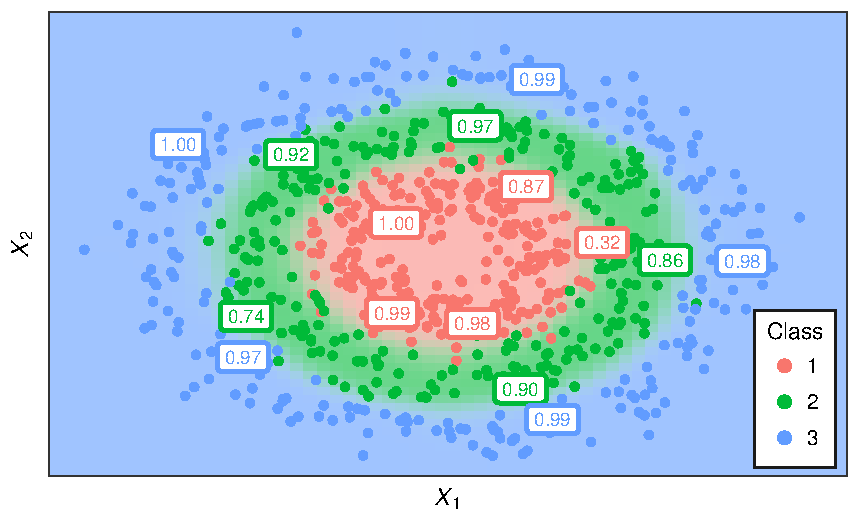
\includegraphics[width=\linewidth,height=17cm]{figure/iprobit_multiclass}
  \vspace{-2cm}
  \caption{A toy example of three-class classification using I-priors and the fBm-0.5 kernel over a two-dimensional predictor. Points indicate realisations, while background colours denote predicted classes. Several predicted probabilities for new data are shown too.}
\end{figure}

\end{column}

\end{columns}

\end{column}



%%%%%%%%%%%%%%%%%%%%%%%%%%%%%%%%%%%%%%%%%%%%%%%%%%%%%%%%%%%%%%%%%%%%%%%%%%%%%%%%
%%% FOURTH COLUMN %%%%%%%%%%%%%%%%%%%%%%%%%%%%%%%%%%%%%%%%%%%%%%%%%%%%%%%%%%%%%%
%%%%%%%%%%%%%%%%%%%%%%%%%%%%%%%%%%%%%%%%%%%%%%%%%%%%%%%%%%%%%%%%%%%%%%%%%%%%%%%%
\spacercolumn
\begin{column}{\onecolwid}



% Variable Selection -----------------------------------------------------------
\vspace{1mm}
\begin{block}{Variable Selection for Linear Models}
Model selection can easily be done by comparing likelihoods (empirical Bayes factors). However, with $p$ variables to select, the $2^p$ comparisons could prove intractable with large $p$.
\\~\\[-0.8ex]
For linear models of the form
\[
  (y_1,\dots,y_n)^\top \sim \N_n \Big( \beta_0\bone_n + \sum_{j=1}^p \beta_j X_j, \Psi^{-1} \Big),
\]
\vspace{-8pt}
the prior
\vspace{-8pt}
\[
  (\beta_1,\dots,\beta_p)^\top \sim \N_p(0, \Lambda X^\top \Psi X \Lambda)
\]
is an equivalent I-prior representation of \eqref{eq:normalmodel} in the feature space of $\beta$ under the linear kernel. 
%Indeed, the prior covariance is the (scaled) Fisher information matrix for $\beta$.
\\~\\[-0.8ex]
Gibbs-based methods with are used in order to estimate \emph{posterior model probabilities}
\[
  p(M | \by) \propto \int p(\by|M, \theta) p(\theta|M) p(M) \d\theta
\]
where $M$ is the model index and $\theta$ are model parameters.
\\~\\[-0.8ex]

\vspace{-0.7cm}
\begin{table}
  \caption{Simulation results (proportion of false choices) for experiments in selecting 100 pairwise-correlated variables using I-priors under differing SNR. Our method outperforms methods such as greedy selection, $g$-priors, and regularisation (ridge and Lasso).}
  \vspace{2.5ex}
  \begin{tabular}{l r r r r r}
  \toprule
  &\multicolumn{5}{ c }{\textbf{Signal-to-noise Ratio (SNR)}} \\
  \textbf{False choices\hspace{15.5mm}}
  & \hspace{0.5cm} \textbf{\hspace{3.5mm}90\%} 
  & \hspace{0.5cm} \textbf{\hspace{3.5mm}75\%} 
  & \hspace{0.5cm} \textbf{\hspace{3.5mm}50\%} 
  & \hspace{0.5cm} \textbf{\hspace{3.5mm}25\%} 
  & \hspace{0.5cm} \textbf{\hspace{3.5mm}10\%} \\
  \midrule
  \textbf{0-2}  & 0.93 & 0.92 & 0.90 & 0.79 & 0.55 \\
  \textbf{3-5}  & 0.07 & 0.07 & 0.10 & 0.20 & 0.27 \\
  \textbf{>5}   & 0.00 & 0.01 & 0.00 & 0.01 & 0.18 \\
  \bottomrule
  \end{tabular}
\end{table}  
\vspace{-3mm}

\end{block}



% Conclusion -------------------------------------------------------------------
\setbeamercolor{block alerted title}{fg=white,bg=colgrey} % Change the alert block title colors
\setbeamercolor{block alerted body}{fg=black,bg=white} % Change the alert block body colors

\begin{alertblock}{Conclusions}

\begin{itemize}
%  \item The EM algorithm provides a straightforward and efficient method of estimating I-prior models.
  \item I-priors provide simple fitting of various regression models for prediction and inference.
  \item The merits of I-priors extend markedly well to the binary and multinomial response case.
  \item Evidence suggests an I-prior advantage for linear variable selection under multicollinearity.
\end{itemize}

\end{alertblock}



% References -------------------------------------------------------------------
\vspace{1mm}
\begin{block}{References}

\vspace{-17pt}
\nocite{*}
\bibliographystyle{unsrt}
\small{\bibliography{bib/phd-poster}}

\end{block}

\end{column}



%%%%%%%%%%%%%%%%%%%%%%%%%%%%%%%%%%%%%%%%%%%%%%%%%%%%%%%%%%%%%%%%%%%%%%%%%%%%%%%%
%%% END DOCUMENT %%%%%%%%%%%%%%%%%%%%%%%%%%%%%%%%%%%%%%%%%%%%%%%%%%%%%%%%%%%%%%%
%%%%%%%%%%%%%%%%%%%%%%%%%%%%%%%%%%%%%%%%%%%%%%%%%%%%%%%%%%%%%%%%%%%%%%%%%%%%%%%%
\spacercolumn
\end{columns} % End of all the columns in the poster
\end{frame} % End of the enclosing frame
\end{document}
